\chapter{Erster Ansatz: Bitcoin}
\label{btc}

\section{Grundlagen}
\iffalse
Kryptowährungen sind digitale Währung, die dezentral organisiert sind. Sie kommen dank Kryptographie ohne das Vertrauen in eine zentrale Stelle aus. Die Idee der digitalen Währungen existiert bereits seit der Erfindung des Internets. Die am 03. Januar 2009 gestartete  digitale Währung ''Bitcoin'' schaffte es erstmalig gänzlich auf die Verwendung einer zentralen Instanz zu verzichten und somit ein verteiltes, dezentrales und sicheres digitales Zahlungssystem zu realisieren.
Bitcoin wurde in dem von dem Pseudonym ''Satoshi Nakamoto'' veröffentlichen Paper ''Bitcoin: A Peer-to-Peer Electronic Cash System'' das erste Mal beschrieben. 
Da der Source Code der Bitcoin Software öffentlich verfügbar ist, hat es seit 2009 eine regelrechte Explosion neuer Kryptowärungen gegeben.
Derzeit gibt es über 1000 verschiedene Kryptowährungen, die auf den Grundprinzipien von Bitcoin aufbauen. 
Grundlegende Komponenten von Kryptowährungen sind:

\begin{itemize}
\item Einem dezentralen Peer-to-Peer Netzwerk, dass mit Hilfe eines währungsspezifischen Protokolls kommuniziert.
\item Der Blockchain, die eine öffentlichen Transaktionsdatenbank darstellt, die alle validen Transaktionen seit dem Start des Netzwerkes aufzeichnet.
\item Eine Menge an Konsensregeln mit Hilfe derer Netzwerkteilnehmer eigenständig Transaktionen auf ihre Richtigkeit prüfen können.
\item Ein Proof-of-Work Algorithmus der es erlaubt, sich in dem globalen dezentralen Netzwerk auf den Zustand der Transaktionsdatenbank zu einigen. Das kontinuierliche Ausführen des Proof-of-Work Algorithmus wird Mining genannt.
\end{itemize}

Die in dieser Arbeit zur Implementierung der Glücksspielanwendung herangezogenen Kryptowährungen bestehen aus diesen Komponenten.


\subsection{Peer-to-Peer Netzwerk}
Peer-to-Peer-Netzwerke sind Netzwerke, die auf direkten Verbindungen zwischen Rechnern beruhen, ohne dass dabei einer der Rechner eine Sonderstellung einnimmt oder ein Server die Kommunikation vermittelt. Quelle: http://www.iwan2002.org/peer.html
In einem reinen Peer-to-Peer-Netz sind alle Computer gleichberechtigt und können sowohl Dienste in Anspruch nehmen, als auch zur Verfügung stellen.
Quelle: https://de.wikipedia.org/wiki/Peer-to-Peer
Das Peer-to-Peer-Modell ist somit grundlegend verschieden von dem im Internet am häufigsten verwendeten Client-Server-Modell. Da jeder Knoten des Netzwerks gleichzeitig Client und Server ist, gibt es keine zentrale Instanz die einen sogenannten ''Single Point of Failure'' darstellt. 

\begin{figure}
\centering
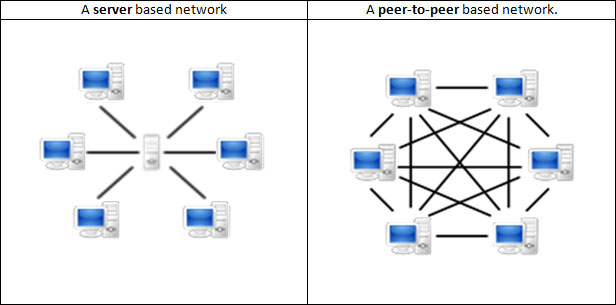
\includegraphics[width=1\linewidth]{Figures/p2p_networks}
\decoRule
\caption{Client-Server | Peer-to-Peer}
\label{fig:p2p_networks}
\end{figure}

Peer-to-Peer Netzwerke sind selbstorganisierend. Das Hinzufügen neuer Teilnehmer und das Entfernen bestehender Netzwerkknoten findet ohne eine zentrale Verwaltung statt und behindert die Funktionsweise des Netzwerks nicht. Jeder Knoten des Netzwerks verwaltet eigenständig seine direkten Nachbarknoten.
Die Art und Weise wie die Teilnehmer des Netzwerkes miteinander Kommunizieren ist durch das Netzwerkprotokoll vorgegeben. Um am Netzwerk teilzunehmen braucht man nur eine Software, die das Netzwerkprotokoll implementiert und einen Internetanschluss.
Im Falle der Kryptowährungen nennt man die Software ''Wallet'' (englisch für Brieftasche), da man mit ihr Zahlungen initiieren und empfangen kann.
Da solch eine ''Wallet'' Software bereits für Smartphones existiert sind die Eintrittsbariren verschwinden gering.

\begin{itemize}
\item Überweisung: Möchte ein Teilnehmer A eine Währungseinheit an einen Teilnehmer B senden, erstellt er dazu eine Nachricht die solch eine Transaktion beeinhaltet und schickt sie an seine direkten Nachbarn. Die Nachbarn prüfen die Gültigkeit der Transaktion mit Hilfe der Konsensregeln und leiten diese gegebenenfalls ah ihre Nachbarn weiter.
\item Neuer Block: Falls ein Teilnehmer des Netzwerk unter Aufwendung von Rechenleistung (Proof-of-Work) einen euen Block von Tansaktionen errechnet hat, broadcaset dieser diesen in Form einer Nachricht an das gesamte Netzwerk.
\end{itemize}

Das DASH Netzwerk besteht im Gegensatz zum Bitcoin aus 2 verschiedenen Knotengruppen. Statt der normalen Full Nodes gibt es zusätzlich sogenannte Masternodes, die besondere Anforderungen (Hardware und 1000 DASH) haben 

%\textcolor(red){\textbf{Hier Bitcoin im ISO OSI Referenzmodell zeigen welche Protokolle auf den verschiedenenen Ebenen genutzr werden. }} Ich denke UDP/IP

%----------------------------------------------------------------------------------------

\subsection{Blockchain}

Eine Blockchain ist eine global verteilte Transaktionsdatenbank. Jeder Teilnehmer des Peer-to-Peer Netzwerkes speichert lokal eine Kopie dieser Datenbank. Dies erlaubt es ihm jegliche Datenbankeinträge zu lesen.
Im Gegensatz zum lesenden Zugriff ist der schreibende Zugriff auf die Datenbank nur unter sehr strikten Regeln möglich. Über diese Regeln sind sich alle Teilnehmer des Netzwerkes einig. Daher werden diese Regeln Konsensregeln genannt. Möchte ein Teilnehmer eine Transaktion in die Datenbank schreiben, muss er sicherstellen, dass sie den Konsensregeln entspricht. Falls die Transaktion eine Konsensregel bricht wird sie vom Netzwerk verworfen und es ist ausgeschlossen, dass Sie in die Blockchain aufgenommen wird. Eine Transaktion beschreibt den Übergang von einem alten Systemzustand in einen neuen Systemzustand.
Im Fall von Bitcoin handelt es sich bei dem Systemzustand um ein digitales Kontenbuch. Eine Transaktion ist in diesem Fall die simple Überweisung eines Betrags von einem Konto A auf ein Konto B. 
Statt eines digitales Kontobuchs kann der Systemzustand allerdings auch wesentlich komplexer sein. Bei der Ethereum Blockchain beinhalten Transaktionen beispielsweise sogenannte ''Smart Contracts''. Dies sind Code-Stücke die es erlauben den Systemzustand auf eine wesentlich komplexere und mächtigere Art und Weise zu verändern.
Möchten mehrere Teilnehmer den Systemzustand durch Transaktionen gleichzeitig anpassen, spielt die Reihenfolge in der die Transaktionen ausgeführt werden eine wichtige Rolle.
%Beispielsweise ist die Überweisung von einem Konto A auf ein Konto B und die anschließende Überweisung von Konto B auf Konto C nicht zwingend in der umgekehrten Reihenfolge möglich.
Transaktionen werden in sogenannten Blöcken, in einer festen Reihenfolge, aggregiert. Somit werden nicht einzelne Transaktionen, sondern ganze Blöcke von Transaktionen in die Datenbank geschrieben.
Genau wie bei den Transaktionen gibt es auch für Blöcke gewisse Konsensregeln. Sobald ein Block allen Konsensregeln entspricht, ist er bereit in die Datenbank aufgenommen zu werden.
Da sich alle Netzwerkteilnehmer über die Gültigkeit des Blockes einig sind, wird somit die globale Blockchain Datenbank angepasst.
Genau wie den Transaktionen ist auch die Reihenfolge der Blöcke wichtig. Daher beinhaltet jeder Block den Hash-Wert seines Vorgängers. Dadurch wird festgelegt auf welchen Block dieser aufbaut.
Durch diese Verkettung der Blöcke, entsteht die sogenannte Blockchain, zu deutsch ''Blockkette''(siehe \ref{fig:blockchain_ETH_white_paper}).
Am Anfang der Kette befindet sich der sogenannte Genesis Block. Auf diesen bauen alle weiteren Blöcke auf.
Nachträgliche Änderungen an einem bereits eingefügtem Block sind nicht möglich, da sich dadurch der Blockhash des Blocks verändert und somit an dieser Stelle die Kette ''zerbricht''.

\begin{figure}
\centering
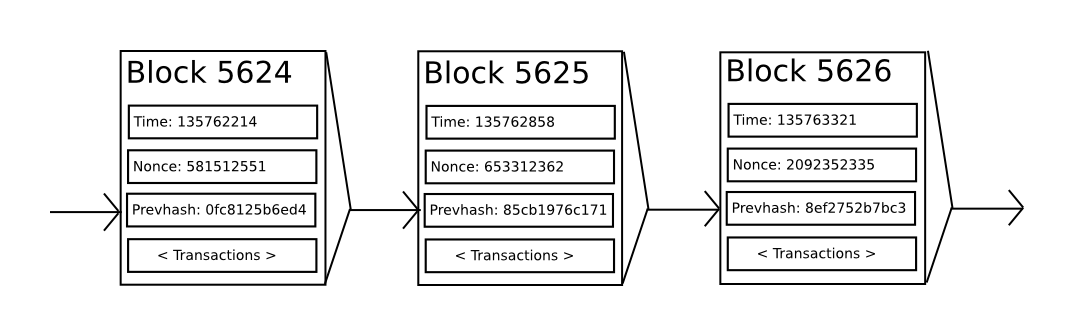
\includegraphics[width=1\linewidth]{Figures/blockchain_ETH_white_paper}
\decoRule
\caption[Kette von Blöcken]{Verkettung von Blöcken.}
\label{fig:blockchain_ETH_white_paper}
\end{figure}



\subsection{Konsensregeln}

Konsenzregeln sind Regeln über die sich alle Teilnehmer des Peer-to-Peer-Netzwerks einig sind. Sie stellen sicher, dass die grundlegenden Eigenschaften der Kryptowährung eingehalten werden. Protokollregeln legen die Syntax der ausgetauschten Nachrichten fest. Konsensregeln legen dagegen die Semantik der ausgetauschten Nachrichten fest. 
Konsensregeln sind den Protokollregeln übergeordnet. Dies bedeutet, dass eine laut Protokollregeln korrekt aufgebaute Transaktionsnachricht, dennoch eine ungültige Transaktion enthalten kann, die den Konsensregeln widerspricht.
Man kann die Konsensregeln in mehrere Kategorien unterteilen.
\subsubsection{Transaktionen}

\begin{itemize}
\item Transaktionen dürfen kein Geld aus dem nichts schöpfen, sondern nur bereits existierende Beträge von einer Adresse auf eine andere Adresse überweisen. Zu dieser Konsensregel gibt es genau eine Ausnahme: die Blockreward-Konsensregel. Diese legt fest wie neue Kryptowährungseinheiten erschaffen werden.
\item Transaktionen, die Geld von Konto A nach Konto B überweisen, müssen durch eine Signatur beweisen, dass sie von dem rechtmäßen Besitzer von Konto A getätigt werden.
\end{itemize}

\subsubsection{Blöcke}

\begin{itemize}
\item Hashing Algorithmus: Mit welcher Kryptografischen Hashfunktion werden Böcke gehasht um sie gegen nachträgliche Modifikation zu schützen? 
\item Blocktzeit: In Abstand von durchschnittlich wie vielen Minuten ist es erlaubt einen Neuen Block in die Blochain einzufügen?
\item Blockgröße? Wie viele Transaktionen darf ein Block beinhalten? Beziehungsweise aus wie vielen Bytes darf ein Block maximal bestehen? 
\item Blockreward: Ein neuer Block darf genau eine Transaktion enthalten, die neue Kryptowährungseinheiten (z.B. 50 Bitcoin) aus dem nichts erschafft. Sowohl die Höhe des Betrags als auch die Anpassung über die Zeit ist in den Konsensregeln des Protokolls hart verankert. Bei Bitcoin beispielsweise halbiert sich der Blockreward alle 4 Jahre. Dies stellt sicher, dass es eine feste Obergrenze an Währungseinheiten gibt.
\item Blocksize: Diese Konsensregel legt die maximale Größe eines Blocks in Megabyte fest. Sie beeinflusst  wie viele Transaktionen in einem Block gebündelt werden können. Die Blocksize Konsensregel ist wichtig, da sie das Wachstum der Blockchain-Datenbank steuert. 
\item Genesis Block: Wie sieht der Hashwert des Genesis-Blocks aus? 
\item Längste Kette: Teilnehmer des Peer-to-Peer Netzwerks folgen immer der längsten Blockkette. 
\end{itemize}

\subsection{Mining}

Teilnehmer, die unbestätigte Transaktionen empfangen, diese in Blöcke zusammenfassen und unter Zuhilfenahme des Proof-of-Work Algorithmus in die Blockchain einfügen werden ''Miner'' genannt.

Dies ist der Fall, da bei diesem rechenintensiven Prozess neue Kryptowährungseinheiten erschaffen werden.

Hier dann auch ein bisschen über die Game Theory schreiben, dass durch einen steigenden Preis der Währung auch mehr Leute Minen und daher merhr echte Ressourcen verschwenden und somit das Netzwerk unangreifbarer machen.

Die Sicherheit des Bitcoin Netzwerkers und die Unmanipulierbarkeit der Blockchain ergeben sich aus der im Protokoll verankerten Spieltheorie (Game Theory). Die Spieltheorie macht es für einen Miner profitabler sich an die Spielregeln des Protokolls zu halten als zu versuchen das Netzwerk zu betrügen. Dies kommt daher, dass Miner Güter aus der echten Welt verbrauchen um sich am Netzwerk zu beteiligen. Falls Miner den sogenannten Blockreward erhalten möchten, müssen sie sich den Spielregeln des Protokolls unterwerfen. Versucht ein Miner einen Block zu produzieren, der den Konsensregeln widerspricht, wird dieser vom Netzwerk verworfen. Somit hält kein anderer Netzwerkteilnehmer den vom Miner an sich selbst ausgeschütteten Blockreward für gültig. Da der Miner aber Ausgaben in Form von Hardwareabnutzung und Stromkosten zu bezahlen hat, schafft dies einen Anreiz sich den Konsensregeln zu unterwerfen.
Die Miner investieren in Hardware und müssen die beim Mining anfallenden Stromkosten bezahlen um unter Aufwendung von Rechenleistung gültige Blöcke zu erzeugen. 
Das Mining ist ein sich selbst regulierendes System bei dem die Anzahl Miner bzw die Hashpower sich mit dem Wert der Kryptowährung anpasst. Steigt der Dollar Preis pro Kryptowährungseinheit, kommen neue Miner zum Netzwerk hinzu und machen das Netzwerk  sicherer. Ein sinkender Preis hat zur Folge, dass der Blockreward nicht mehr für die Bezahlung der Strom und Hardwarekosten ausreicht. Dies hat zur Folge, dass die Anzahl an Miner abnimmt. Somit sinkt auch die Sicherheit des Netzwerks.

\fi